\chapter{Fundamentação Teórica}
\label{cap:fundamentacao-teorica}

Neste capitulo é apresentado uma pesquisa envolvendo os principais fundamentos envolvidos no desenvolvimento do jogo.

\section{Os Gêneros dos Jogos}
\label{sec:os-generos-dos-jogos}

Gênero de jogo pode ser definido como uma modalidade ou tipo que permite o agrupamento de diversos jogos de acordo com suas características de jogabilidade.
Segundo Eucidio, pensar no jogo é pensar no estilo de produção que o jogo seguirá, pensar nos desafios, dificuldades e possibilidades. \cite{euc}

A plataforma dos jogos também influenciam para determinar o gênero do jogo. Em smartphones, por exemplo, os jogos tendem a ser mais casuais e rápidos. Existe uma infinidade de categorizações. \cite{gen}

\begin{alineascomponto}
\item Jogos de Ação\\
Significa atividade, agir de acordo com  situação. O jogador tem que tomar alguma ação em tempo real, agindo rapidamente. Jogos deste gênero é o mais popular para a plataforma PC. Um exemplo de jogo de ação é o Half-Life 2, onde possui as características de ser um jogo sagaz, envolvente e com enredo, na figura 3 encontra-se a capa da Mídia digital deste jogo. \cite{gen1}
\end{alineascomponto}
\begin{figure}[h!]
		\centering
		\Caption{\label{fig:exemplo-4}Jogo Half Life 2, desenvolvido pela Valve Corporation (2004)}	
		\UECEfig{}{
			\fbox{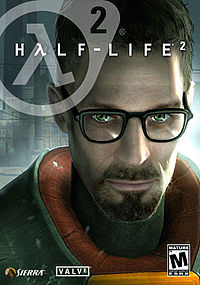
\includegraphics[width=5cm]{figuras/HalfLife}}
		}{
			\Fonte{\cite{hl}}
						
		}	
	\end{figure}
\begin{alineascomponto}
\item Jogos de Simulação\\
É a representação da realidade, são jogos que simulam situações vividas por seres humanos. A principal utilização por este gênero é para simulação de voos, tendo como objetivo o treinamento de pilotos, como por exemplo, o jogo FlightSimulator da Microsoft. Na figura 4 é possível ver a simulação que ocorre no jogo. \cite{gen1}
\end{alineascomponto}
\begin{figure}[h!]
		\centering
		\Caption{\label{fig:exemplo-5}Jogo Flight Simulator desenvolvido pela Microsoft (2015)}	
		\UECEfig{}{
			\fbox{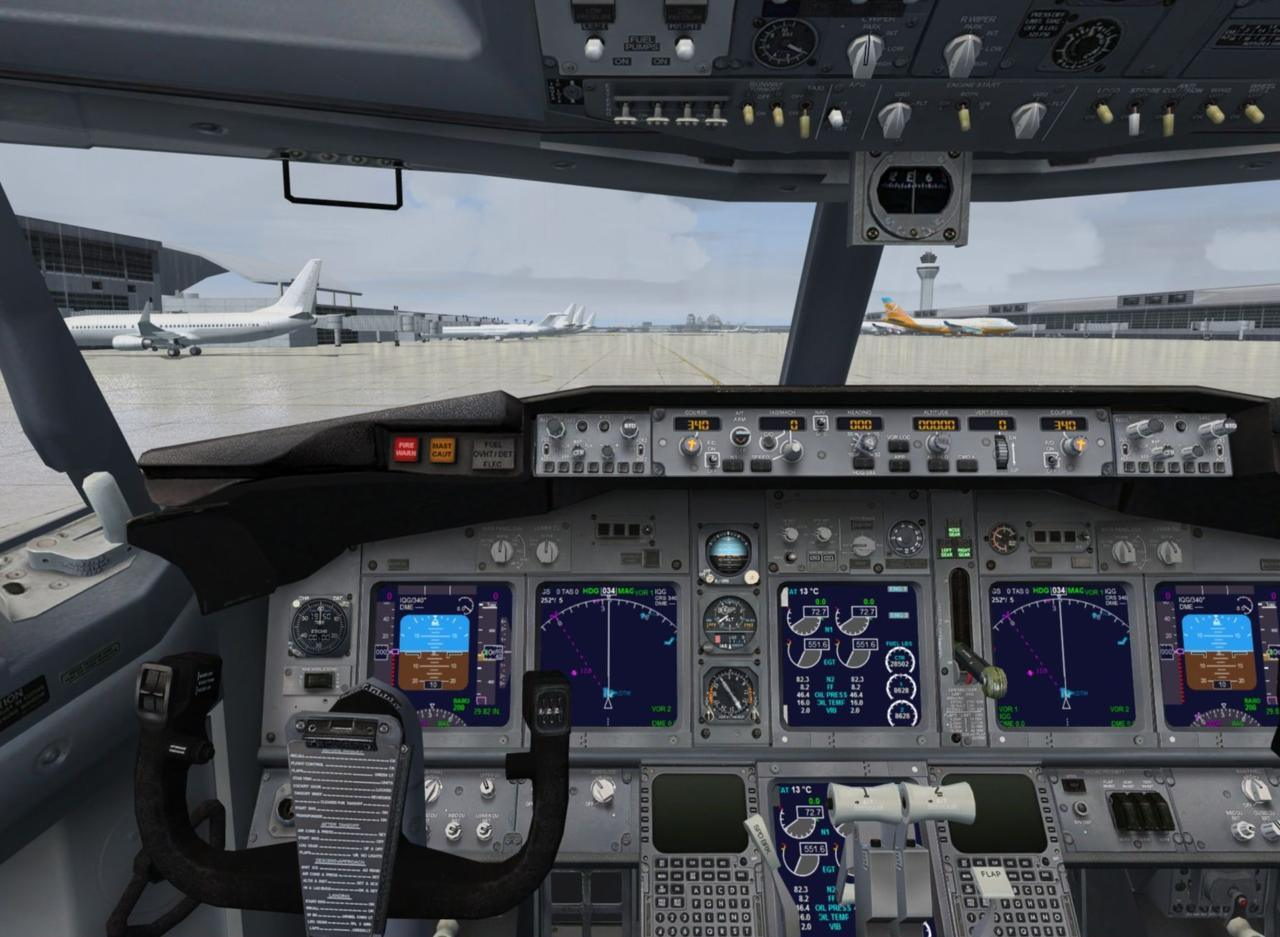
\includegraphics[width=7cm]{figuras/MFS}}
		}{
			\Fonte{\cite{fs}}			
		}	
	\end{figure}

\begin{alineascomponto}
\item Jogos de RPG\\
Tem como característica o desenvolvimento gradativo do personagem. O jogador assume o papel do personagem aonde pode haver narrativas para auxiliar no decorrer do jogo.
Um jogo muito conhecido que utiliza deste gênero é o Final Fantasy XIII,  na figura 5 encontra-se a capa da Mídia digital deste jogo. \cite{gen1}
\end{alineascomponto}
\pagebreak
\begin{figure}[h!]
		\centering
		\Caption{\label{fig:exemplo-6}Jogo Final Fantasy XIII desenvolvido pela Square Enix (2009)}	
		\UECEfig{}{
			\fbox{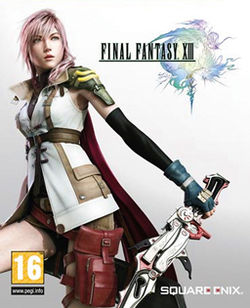
\includegraphics[width=6cm]{figuras/FF}}
		}{
			\Fonte{\cite{ff}}			
		}	
	\end{figure}
	
\begin{alineascomponto}
\item Jogos de Esportes\\
A principal característica de jogos deste gênero é que o controle ocorre sobre o personagem não mecânico. Normalmente o jogo tem um esforço físico do jogador no mundo virtual, em alguns jogos o personagem cansa e diminui sua velocidade. Um exemplo de jogo de esporte é o FIFA, conforme demostrado na figura 6. \cite{gen1}

\end{alineascomponto}
\begin{figure}[h!]
		\centering
		\Caption{\label{fig:exemplo-7}Fifa 15 desenvolvido pela EA Sports (2014)}	
		\UECEfig{}{
			\fbox{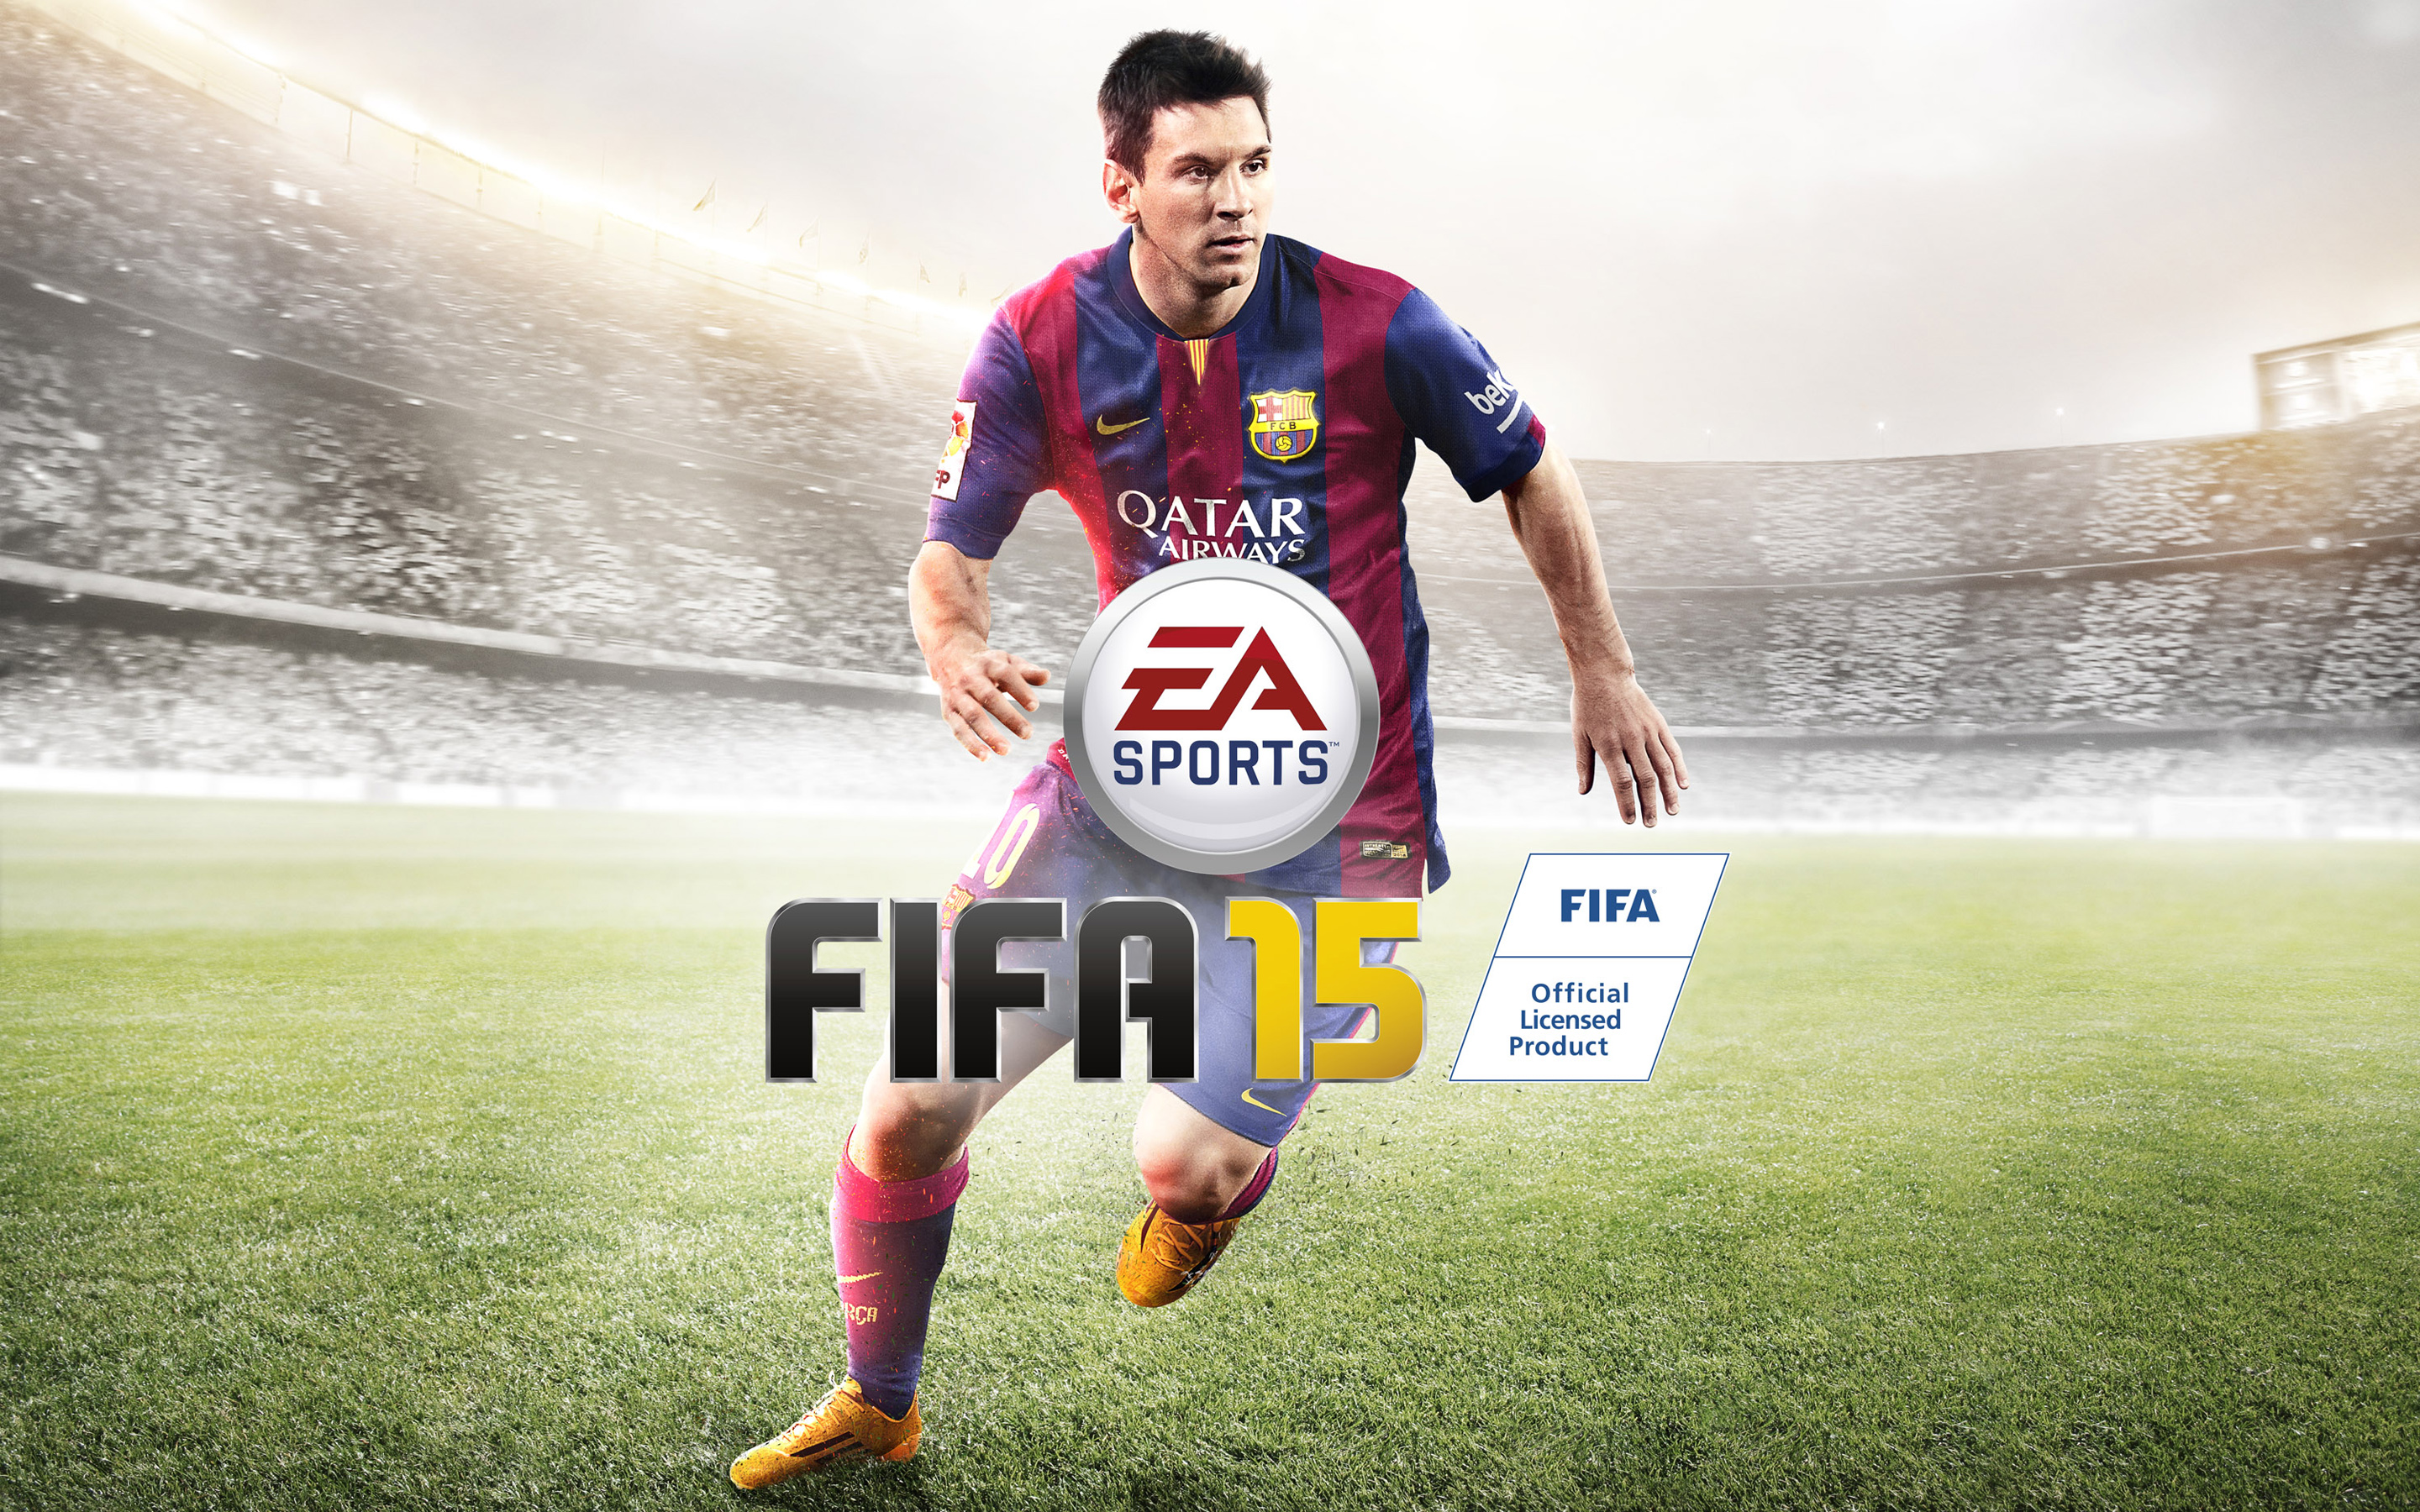
\includegraphics[width=7cm]{figuras/Fifa15}}
		}{
			\Fonte{\cite{fifa}}			
		}	
	\end{figure}
	
\pagebreak
\begin{alineascomponto}	
\item Jogos Educacionais\\
São jogos que possuem o intuito de ensinar as pessoas sobre determinado assunto, reforçando assim seu desenvolvimento e entendimento sobre um evento histórico ou cultural, ou ainda auxiliar na aprendizagem de alguma habilidade enquanto de joga. \cite{jd}

\end{alineascomponto}

\section{Categoria de Jogos}
\label{sec:categoria-de-jogos}

É possível classificar os jogos em 3 categorias, sendo estas:
\begin{alineascomponto}

\item Jogos 2D\\
Implementados a partir de gráficos bidimensionais somente com uma camada.

 Perspectiva \textit{ Top-down} - tem a perspectiva sobre a cabeça do personagem e este pode se movimentar em qualquer ângulo.
 \textit{Side Scroling} - tem a perspectiva do lado do personagem onde este se move para direita ou esquerda, comum em jogos de plataforma. Na figura 7 é possível verificar a representação gráfica de um plano 2D (bidimensional). \cite{graf}

\end{alineascomponto}


\begin{figure}[h!]
		\centering
		\Caption{\label{fig:exemplo-}Representação gráfica de um plano bidimensional}	
		\UECEfig{}{
			\fbox{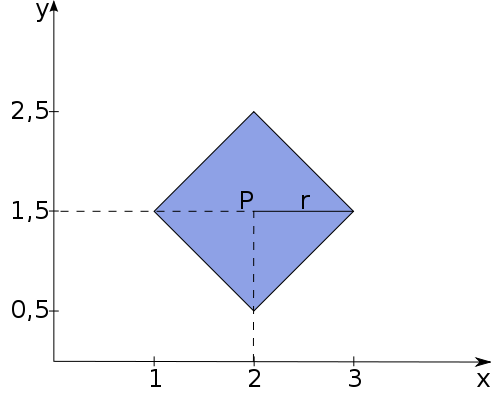
\includegraphics[width=7cm]{figuras/2D}}
		}{
			\Fonte{\cite{2d}}			
		}	
	\end{figure}

\begin{alineascomponto}


\item Jogos 2.5D\\
Atribuído em jogos onde o 2D e o 3D são combinados para reproduzir um cenário mais realista. Nesta categoria os personagens são modelados em imagens 2D e se movimentam em um cenário 3D ou um personagem em 3D em um fundo 2D, porém sendo mais comum um cenário que apresenta características de dimensão de profundidade a partir da sobreposição de imagens 2D.

Se divide na categorias: Isométrico, projeção oblíqua, \textit{billboarding} e escalamento do eixo Z. Na figura 8 é possível verificar a representação gráfica de um plano 2.5D (isométrico). \cite{graf}

\end{alineascomponto}

\begin{figure}[h!]
		\centering
		\Caption{\label{fig:exemplo-4}Representação gráfica de um espaço isométrico (2.5D)}	
		\UECEfig{}{
			\fbox{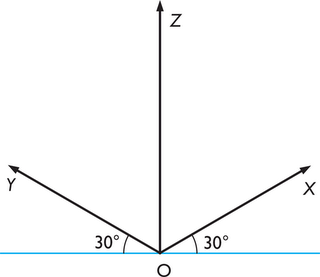
\includegraphics[width=7cm]{figuras/isometrico}}
		}{
			\Fonte{\cite{25d}}			
		}	
	\end{figure}
	
\begin{alineascomponto}

\item Jogos 3D\\
São jogos onde o cenário é modelado tridimensionalmente sendo possível o personagem mover-se em qualquer direção.
Se dividem nas categorias
\begin{alineascomponto}
\item 3D Fixo - Jogo onde a câmera é fixa.
\item Primeira pessoa - Jogo onde a câmera está na posição na altura dos olhos do personagem.
\item Terceira pessoa - Jogo aonde câmera está próxima ao personagem, sempre o acompanhando. 
\end{alineascomponto}
Na figura 9 é possível verificar a representação gráfica de um plano 3D (tridimensional). \cite{graf}
\end{alineascomponto}
\pagebreak
\begin{figure}[h!]
		\centering
		\Caption{\label{fig:exemplo-7}Representação gráfica de um espaço tridimensional}	
		\UECEfig{}{
			\fbox{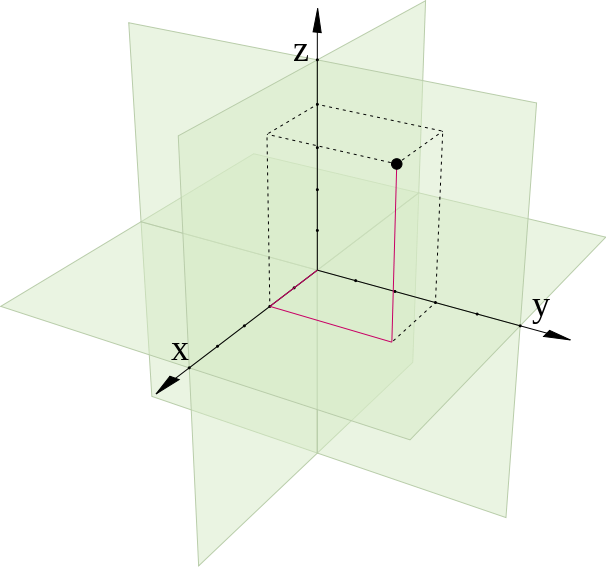
\includegraphics[width=7cm]{figuras/3D}}
		}{
			\Fonte{\cite{3d}}			
		}	
	\end{figure}
	
\begin{comment}

http://www.dca.fee.unicamp.br/~martino/disciplinas/ia369/trabalhos/t3g1.pdf
https://pt.wikipedia.org/wiki/G%C3%AAneros_de_jogos_eletr%C3%B4nicos
\end{comment}
\section{Engenharia de Software}
\label{sec:engenharia-de-software}

Sommerville  definiu engenharia de software como uma disciplina da engenharia que cuida de todos os aspectos da produção de software, desde a especificação do sistema até a sua manutenção, depois que ele entra em operação.

A engenharia é constituída de processos de software, que são conjuntos de atividades e resultados para se produzir um software. Existem quatro atividades fundamentais, são elas: 
\begin{alineascomponto}

\item Especificação de Software: o software a ser desenvolvido e as restrições para sua operação são definidos. 
Desenvolvimento de Software: o software deve ser feito atendendo suas especificações.
\item Validação de Software: o software tem de ser validado para garantir que está em cima do que o cliente deseja. 
\item Evolução do Software: o software sofre modificações para atender as necessidades do cliente. \cite{somm}
\end{alineascomponto}

No desenvolvimento de software, o principal objetivo é a criação de sistemas que atendam às necessidades dos clientes e usuários, ou seja, uma correta especificação dos requisitos se torna essencial para que o desenvolvimento tenha sucesso. Uma forma de entender melhor esses requisitos é dividindo-os em: Requisitos Funcionais e Requisitos Não-Funcionais. 


Os Requisitos Funcionais definem as funções que componentes do sistema ou sistemas devem executar. 
Os Requisitos Não-Funcionais incluem limitações no produto, como por exemplo: desempenho, confiabilidade, segurança e limitações no desenvolvimento, como custos e tempo, componentes a serem reutilizados, entre outros. \cite{vac}

\section{Desenvolvimento Mobile}
\label{sec:desenvolvimento-mobile}

Um dispositivo móvel pode ser definido como um computador de bolso, normalmente composto de uma tela e um teclado em miniatura podendo estes serem combinados em um só dispositivo conhecido como \textit{ touchscreen}.

Características dos dispositivos móveis:

\begin{alineascomponto}
 
\item Pequeno em tamanho
\item Baixo consumo de energia
\item Curto tempo de inicialização
\item Armazenamento de dados local e/ou remoto

	\end{alineascomponto}


Os dispositivos móveis mais populares são:

\begin{alineascomponto}
 
\item \textit{Smartphone}
\item \textit {Tablet}
\item Console portátil
\item \textit {Notebook}

	\end{alineascomponto}
	\cite{mov}
	\begin{comment} 
	http://www.dca.fee.unicamp.br/~martino/disciplinas/ia369/trabalhos/t1g1.pdf

https://books.google.com.br/books?id=pWc3AgAAQBAJ&pg=PA46&lpg=PA46&dq=estilo+de+jogos+digitais&source=bl&ots=P8i8N4DcJL&sig=uj-5ewjDs8v_Ea5XAtmdELqSQMY&hl=pt-BR&sa=X&ved=0ahUKEwj85cSisLvJAhWON5AKHXH-CAEQ6AEIWDAJ#v=onepage&q=estilo%20de%20jogos%20digitais&f=false
\end{comment}

A tecnologia que torna viável a existência dos dispositivos móveis começou a partir do primeiro celular inventado, em 3 de abril de 1983, o Motorola DynaTAC 8000x. Foi então que em 1992 a empresa Apple lançou no mercado o primeiro PDA que continha memória de 1MB e tela sensível ao toque, desde então esta tecnologia tem se desenvolvido e mostrado como vantagem  a possibilidade dos dados serem acessados em qualquer lugar a qualquer hora. \cite{1cel}

Dentre os dispositivos móveis citados, o que mais se destacam são os \textit{smartphones}. Um \textit{smartphone} (telefone inteligente) poder ser definido como um celular que possui muitas funções. Essas funções são realizadas de maneira mais eficientes do que em um celular normal, em geral possuem internet wiFi, navegadores, assim como também é possível realizar a instalação de aplicativos e possui um Sistema Operacional (SO). \cite{smar} 

Um Sistema Operacional é um conjunto de programas responsável por alocar recursos do hardware fornecendo também uma interface para o usuário. Os sistemas operacionais para smartphones mais conhecidos atualmente são: iOS, Android, Windows Mobile e BlackBerry \cite{oqsmar}

Segundo uma pesquisa realizada pela Gartner, o sistema operacional mais vendido em 2015 (para \textit{smartphones}) foi o Android e em segundo o iOS, conforme pode ser visto na figura 10. \cite{gar}
\begin{figure}[h!]
		\centering
		\Caption{\label{fig:exemplo-1}Venda Mundial de Smartphones por Sistemas Operacionais}	
		\UECEfig{}{
			\fbox{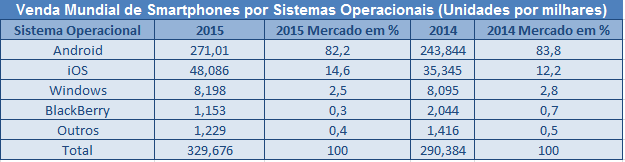
\includegraphics[width=13cm]{figuras/GartnetSamart}}
		}{
			\Fonte{Gartner, 2015}			
		}	
	\end{figure}

\subsection{Aplicativos Móveis}
Um aplicativo móvel, conhecido também como App é um software desenvolvido para dispositivos móveis, por exemplo, \textit{smartphones},  \textit{Tablets}, \textit{notebboks}, esses aplicativos podem ser nativos, Web ou híbridos. \cite{dif}

\begin{alineascomponto}

\item Aplicativos Nativos

São os aplicativos que podem ser acessados na tela principal através de seu ícone. Podem ser instalados através de um aplicativo de loja específico para sua plataforma, como por exemplo o sistema iOS utiliza a App Store baixar seus aplicativos, enquanto o Android utiliza o Google Play. Esses aplicativos residem no dispositivo.

\item \textit{Mobile Web Apps}

São aplicativos que na verdade são sites e não aplicativos raiz, como os nativos. São executados a partir de um navegador e normalmente criado um ícone na tela principal do dispositivo para que quando clicando ele acesse a URL determinada.

\item Aplicativos Híbridos

São os aplicativos que são parcialmente web e nativos.
Estes devem ser baixados pela loja de aplicativos, ficam armazenados no dispositivo porém podem também serem utilizado como web App.

	\end{alineascomponto} 
	
Segundo dados divulgados pelo Ministério de Ciência Tecnologia e Inovação (MCTI), o mercado de aplicativos móveis está em alta, movimentando mais de US\$ 25 bilhões por ano no Brasil, com expectativas de alcançar US\$ 70 milhões até 2017. \cite{mcti}
	
	
	\begin{comment}
http://www.luisaambros.com/blog/diferenca-entre-aplicativos-nativos-hibridos-e-mobile-web-apps/

http://www.correiobraziliense.com.br/app/noticia/tecnologia/2015/05/11/interna_tecnologia,482694/brasil-decola-na-industria-de-apps-e-mercado-acumula-lucros-nesta-deca.shtml
\end{comment}
	
\begin{comment}
http://www.telefonescelulares.com.br/o-que-e-smartphone/
http://pt.slideshare.net/cetorres/palestra-mobilidade-computao-mvel-dispositivos-e-aplicativos-2013
\end{comment}

\section{Android}
\label{sec:Android}
Android é um sistema operacional para dispositivos móveis, seu código é aberto (\textit{open-source}). Inicialmente desenvolvido pela Android Inc, em 2003 comprada pela empresa Google e desde 2007 mantida pela \textit{Open Handset Alliance} (OHA).

O sistema operacional Android possui seu núcleo (\textit{Kernel}) em Linux e utiliza Java como linguagem de programação padrão. Também utiliza de sua própria maquina virtual chamada de Dalvik.

A máquina virtual Dalvik possui grandes diferenças entre a Java Virtual Machine (JVM) tornndo-a superior; a Dalvika é baseada em registradores e não em pilhas como a JVM.

A Dalvika executa seus arquivos na extensão ".dex" (Dalvik Executable) que nada mais são do que arquivos Java já previamente projetados e compilados realizando a otimização de memoria e compartilhamento de dados.

Na figura 11 é possível fazer um comparativo entre a JVM (.class) e a Dalvik VM (.dex). \cite{desa}

\pagebreak
\begin{figure}[h!]
		\centering
		\Caption{\label{fig:exemplo-2}Comparação do formato .class da JVM com o .dex usado pela Dalvik VM.}	
		\UECEfig{}{
			\fbox{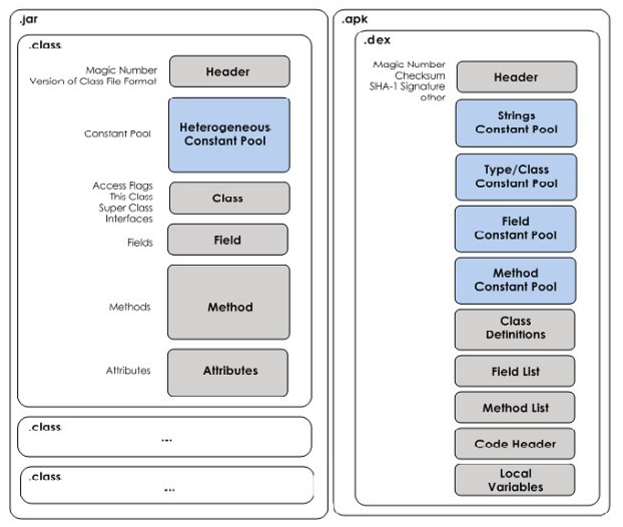
\includegraphics[width=13cm]{figuras/JvmDvm}}
		}{
			\Fonte{Marcelo Korjenioski, 2011}			
		}	
	\end{figure}

\subsection{Google Play }

Google Play também conhecida como Google Play Store é a loja virtual da Google para venda de aplicativos. Antigamente esta loja virtual recebia o nome de Android Market mas em 2012 seu nome mudou para haver a unificação de produtos.
No Google Play esta disponível para usuário baixar aplicativos gratuito e/ou pagos. \cite{gp}

\begin{comment}http://smartmundo.com/o-que-e-play-store/
\end{comment}
Para um desenvolvedor distribuir seus aplicativos na Google Play é necessário que o mesmo faça seu cadastro e pague uma quantia de U\$25,00, feito isso será possível fornecer seu aplicativo na loja virtual. Uma vez que o desenvolvedor tem a conta criada é possível ter acesso a comentários, estatísticas e erros de seus aplicativos. Caso o aplicativo seja pago, o lucro para o desenvolvedor é de 70\% do valor cobrado pelo aplicativo. \cite{tt}
\begin{comment}http://www.tutoriandroid.com/2012/05/como-publicar-no-google-play.html
\end{comment}

\subsection{Versões Disponíveis}

Desde de seu inicio, o Android nomeia suas versões com nomes de doces e sobremesas e segue uma ordem alfabética. Ainda não foi revelada pela empresa o real motivo deste padrão de nomenclatura.

Atualmente existem 13 versões do sistema operacional Android, estes apresentados na tabela 1. \cite{vs}

\begin{comment}
http://www.aplicativosandroid.com/conhecam-todas-as-versoes-do-android-e-seus-maravilhos-doces/3891 ---  e tabela ----- http://www.tecmundo.com.br/android/82344-linha-tempo-dentro-evolucao-do-sistema-android.htm
\end{comment}


\begin{table}[h!]
	\Caption{\label{tabela-android} Tabela contendo nome, versão e ano de lançamento dos sistemas Androids.}%
	\IBGEtab{}{%
		\begin{tabular}{ccc}
			\toprule
			Nome & Versões & Ano de Lançamento \\
			\midrule \midrule
			Alpha (Apple Pie)  & 1.0 & 2008 
			\\
			Beta (Banana Bread) & 1.1 & 2009 \\
			Cupcake & 1.5 & 2009\\
			Donut & 1.6 & 2009 \\
			Eclair & 2.0 e 2.1 & 2009 \\
			Froyo & 2.2 & 2010 \\
			Gingerbread & 2.3 & 2010 \\
			Honeycomb & 3.0; 3.1; 3.2 & 2011 \\
			Ice Cream Sandwich & 4.0 & 2011 \\
			Jelly Bean & 4.1; 4.2; 4.3 & 2012 e 2013 \\
			KitKat & 4.4 & 2013 e 2014 \\
			Lollipop & 5.0 & 2014 e 2015 \\
			Marshmallow & 6.0 & 2015 \\
			\bottomrule
		\end{tabular}%
	}{%
	\Fonte{\cite{doc}}%
}
\end{table}
\pagebreak
\section{Scrum}
\label{sec:scrum}

Segundo Jeff Sutherland, o criador da metodologia, o SCRUM foi criado para ser uma forma mais rápida, eficaz e confiável de criar softwares para o setor de tecnologia. \cite{jeff}

A metodologia apresentada pelo seu co-criado, Ken Schwaber, nos fala que SCRUM é um \textit{framework} na qual possibilita o emprego de diversos processos e técnicas. Ele define também que o papel do Scrum é "fazer
transparecer a eficácia relativa das suas práticas de desenvolvimento para que você possa melhorá-las, enquanto provê um \textit{framework} dentro do qual produtos complexos podem ser desenvolvidos." \cite{Kenn}

O Scrum é formado por um conjunto de Times Scrum com papeis associados, Eventos com duração fixa (Time-Boxes), Artefatos e Regras.

O Time Scrum visa otimizar a produtividade e flexibilidade, e para atingir este fim, o Time é dividido em três papeis.

\begin{alineascomponto}
\item \textit{Scrum Master}

Responsável por garantir que o processo seja entendido e seguido, fazendo com que o Time esteja de acordo com  metodologia Scrum suas párticas e regras, ajudando-os a a entender o auto- gerenciamento e a interdisciplinaridade.

\item \textit{Product Owner}

Responsável por maximizar o valor do trabalho do Time Scrum e também o único responsável pelo gerenciamento do Backlog do Produto garantido que este esteja visível a todos, para que o Time consiga compreender quais itens possuem maior prioridade. 

\item {Time}
	
Executa o trabalho propriamente dito, desenvolvendo o Backlog do Produto entregáveis em cada Sprint. os membros do Time devem possuir total conhecimento necessário pra o desenvolvimento. Os times são auto-organizáveis, nem mesmo o Scrum Master pode interferir e dizer ao time como transformar o Backlog em funcionalidades entregáveis.
O tamanho desejável para um time  é de sete pessoas.
\end{alineascomponto}

A figura 12 apresenta interação entre os papeis.

	\begin{figure}[h!]
		\centering
		\Caption{\label{fig:exemplo-3} Interação entre os papeis }	
		\UECEfig{}{
			\fbox{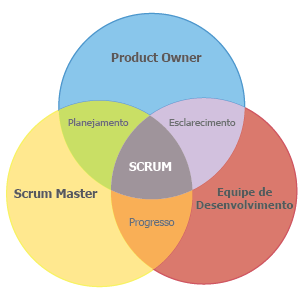
\includegraphics[width=08cm]{figuras/roles}}
		}{
		\Fonte{\cite{int}}			
	}	
	\end{figure}

\subsection{Time-Boxes}
Consiste em Reunião de planejamento, revisão e retrospectiva da Sprint, Sprint e Reunião Diária.

Sprint

São eventos com duração fixa, onde durante o \textit {ScrumMaster} garante que não será feita nenhuma alteração que possa afetar a Meta Sprint. As Sprints consistem na reunião de Planejamento, Revisão e Retrospectiva. Elas também ocorrem sem intervalos, um após outra.

Reunião Diária

O Time se encontra diariamente para reuniões de 15 minutos, visando melhorar comunicação e remover impedimentos no desenvolvimento. Nessas reuniões cada membro explica:

\begin{enumerate}
   \item O que ele realizou desde a última reunião diária;
   \item O que ele vai fazer antes da próxima reunião diária;
   \item  Quais obstáculos estão em seu caminho.
 \end{enumerate}

Backlog do Produto

Representa todas as necessidades para desenvolver e lançar um produto junto com os requisitos do produto que o Time está desenvolvendo, o responsável por ele é o Product Owner.  Backlog vai evolui na mesma proporção que o produtoç ele é flexivel, está constantemente mudando par identificar as necessidades do produto para melhor aprimorá-lo. Enquanto existir o produto, o Backlog do Produto também existirá.

Backlog da Sprint

Consiste em tarefas que o Time executa para transformar itens do Backlog do Produto em um incremento pronto. O Time modifica o Backlog da Sprint durante a Sprint assim quando ocorre as tarefas individuais é possível identificar quais tarefas são necessárias ou que a tarefa pode levar mais ou menos tempo pra ser concluída
.

	
A figura 13 representa o processo de interação das atividades.

	\begin{figure}[h!]
		\centering
		\Caption{\label{fig:exemplo-3} Interação das atividades }	
		\UECEfig{}{
			\fbox{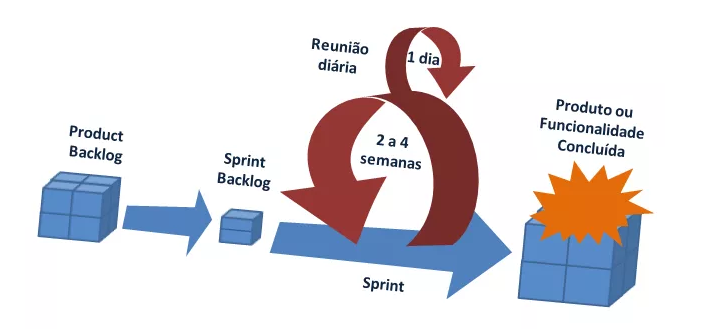
\includegraphics[width=10cm]{figuras/InteracaoScrum}}
		}{
		\Fonte{\cite{scrum}}			
	}	
	\end{figure}
 

\section{Controle de Versão}
\label{sec:Controle-de-Versão}

O controle de versão tem como objetivo a gerencia de versões de um mesmo projeto. Vários programadores podem trabalhar em um mesmo projeto sendo possível manter um histórico de atualizações.

Dentre as infinidades de vantagens para se utilizar um "controlador de versões" as três principais que se destacam são:
\begin{alineascomponto}
	
   \item Possibilidade de salvar o histórico
   \item Possibilidade de desenvolver versões diferentes
   \item Possibilidade de se programar em paralelo

	\end{alineascomponto}
	
	
O controle de versão funciona da seguinte forma: os históricos contendo as modificações de cada versão ficam armazenados em um repositório (servidor). Este processo dá à liberdade para que o desenvolvedor possa baixar a última versão, trabalhar em seu código e posteriormente atualizar a versão já previamente armazenada no servidor, este processo pode ser visto na figura 14.

	\begin{figure}[h!]
		\centering
		\Caption{\label{fig:exemplo-4} Funcionamento do Controle de Versão}	
		\UECEfig{}{
			\fbox{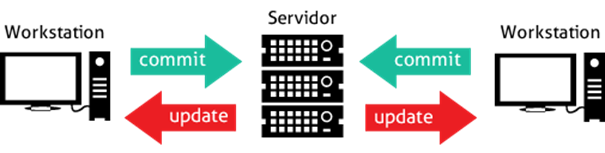
\includegraphics[width=13cm]{figuras/ControleVersao}}
		}{
		\Fonte{\cite{cv}}			
	}	
	\end{figure}
	
	Para que seja realizada a sincronização entre a \textit{workstation} e o servidor é necessário utilizar os comandos:
	
	\begin{alineascomponto}
\item \textit{Commit} - realiza o envio das alterações realizadas para o servidor gerando um novo histórico de atualizações.
\item \textit{Update} - realiza o envio da última versão contida no servidor para a \textit{workstation}.
\cite{cv}
	\end{alineascomponto}
	
	\subsection{Bitbucket}
	
No mercado atualmente existem dois grandes serviços que disponibilizam o controle de versionamento e estes são: Github e o Bitbucket.

Bitbucket é uma ferramente de domínio da empresa Atlassian e implementa dois padrões de versionamentos, o GIT e o Mercurial. \cite{bit}

\section{Inteligência Artificial}
\label{sec:inteligencia-artificial}

A Inteligência Artificial (IA) é um ramo de pesquisa da ciência da computação que procura através de meio computacionais desenvolver mecanismos e/ou dispositivos que simulem a capacidade do ser humano de raciocinar e resolver problemas, ou seja, ser inteligente. 

O campo de IA tem como objetivo, o contínuo aumento da "inteligência" do computador, pesquisando, para isto, os fenômenos da inteligência natural. Para este fim, IA é definida  como sendo uma coleção de técnicas suportadas por computador emulando algumas capacidades dos seres humanos. Esta coleção inclui:

\begin{alineascomponto}
	
   \item Resolução de problemas
   \item Compreensão de Linguagem Natural
   \item Visão e Robótica
   \item Sistemas Especialistas e Aquisição de Conhecimento
   \item Metodologias de Representação de Conhecimento

	\end{alineascomponto}
	
Hoje em dia a Inteligência Artificial é utilizada em vários fins, não só exclusivamente para informática, no entanto, um dos pontos em que se destaca é para o desenvolvimento de jogos. 

Primeiramente utilizada em jogos clássicos como xadrez ou jogo da velha e atualmente utilizada para jogos digitais.

Os algoritmos de IA desenvolvidos para jogos digitais podem ser divididos em três blocos:

\begin{alineascomponto}
	
\item Movimento:

De como um personagem é movimentado, do local inicial até o destino final, também determina o cálculo do percurso, detectando objetos e desviando de obstáculos.
   
 \item Tomada de Decisão:
 
Cada personagem possui um conjunto de atividades e estados possíveis, estes sendo: estar parado, fugir, atacar adversário, entre outros. Para que cada ação seja possível, a personagem precisará fazer uma tomada de decisão analisando o contexto. Esta decisão pode ser de ativar um algoritmo de movimento, alterar um estado interno ou a animação. Não necessariamente essas alterações serão visuais.

\item Estratégia:

A maioria dos jogos digitais desenvolvidos com IA ocorrem nos dois tipos já citados estes também podem conter personagens que trabalham em grupo ou equipe contando com uma tomada de decisão individual.

	\end{alineascomponto}

	
As pesquisas iniciaram-se na Segunda Guerra Mundial, com os cientistas Hebert Simon, Allen Newell,  Jonh McCarthy com o objetivo em comum de reproduzir uma máquina que simulasse o cérebro humano. \cite{ia}

\section{Busca Heurística}
\label{sec:Busca-Heurística}

A busca heurística pode ser definida como uma estratégia que faz uso do conhecimento específico do problema, sendo possível obter soluções mais eficientes do que uma estratégia sem informação. \cite{rus}

De acordo com \cite{el}, heurística é uma técnica eficiente para um processo de busca. A heurística, mesmo que as vezes possa passar por pontos de interesse despercebidos, pode levar a direcionamentos interessantes. A heurística aprimora os caminhos a serem percorridos, entretanto pode desconsiderar o melhorar caminho a percorrer. 


\subsection{Algoritmo A* (A estrela)}	
O A* (lê-se A estrela) é um algoritmo de busca de caminho \textit{(pathfinding)}. Segundo Russel (2003) A* é a forma mais eficiente pela busca da melhor escolha, na qual avalia os nós combinando o custo para alcançar cada nó \textit{g(n)} e o custo do nó ate o objetivo h(n).

\begin{align*}
    \textbf{f(n) = g(n) + h(n)}
\end{align*}


A função \textit{f(n)} representa o custo estimado da solução menos custosa passando por \textit{n} e chegando ao estado-objetivo. O A* utiliza também o método de lista aberta e fechada aonde listas abertas armazenam todos o nós que foram gerados porém ainda não examinados e a fechada armazena os nós que já analisados.

O algoritmo A* é completo e eficiente contanto que a função heurística \textit{f(n)} não superestime o custo ate o estado-objetivo.
\cite{aestar}
\begin{comment}
http://dsc.inf.furb.br/arquivos/tccs/monografias/2005-1jeanitabassanidasilvavf.pdf
file:///C:/Users/Talita/Downloads/601-1351-2-PB.pdf
\end{comment}

\section{Orientação Objeto}
\label{sec:orientação-objeto}	

O termo "Orientação a Objeto" conota o processo de modelar um sistema como "um grupo de agentes autônomos que colaboram para realizar algum procedimento de alto nível".  
Este paradigma possibilita o desenvolvimento de software baseado em objetos, assim como os do mundo real,  que interagem a fim de resolver um determinado problema.  
  
Segundo Daniel Clark , programação orientada a objeto pode ser definida como uma abordagem em desenvolvimento de software em que a estrutura do software é baseada na interação entre objetos para realizar uma tarefa.  
  
Ainda segundo Daniel Clark, os benefícios em utilizar este paradigma seriam: 

  \begin{alineascomponto}
\item Uma transição mais intuitiva dos modelos de análise de negócio para implementação de modelos de software.  
  
\item A Possibilidade de manter e implementar mudanças no programa de forma mais eficiente e rápida.

\item A possibilidade de reuso de componentes de código em outros programas dentre outros. 
\end {alineascomponto}
\cite{dan}

\subsection{Classes e Objetos}	

Como dito na definição de orientação a objetos, objetos e suas interações  são recursos indispensáveis para a existência deste paradigma, neste contexto pode-se definir objeto como uma estrutura que incorpora dados e os procedimentos para trabalhar com estes dados.

Para a construção dos objetos faz-se necessário  um outro recurso, conhecido como Classe que segundo Daniel Clark se entende por uma definição complexa de tipo de dado para um objeto e que ela contém informação sobre como um objeto deveria se comportar, incluindo seu nome, métodos, propriedades e eventos.\cite{dan}


\subsection{Classes Abstratas}	

Segundo Danny Poo, em uma hierarquia de classe há classes que são tão genéricas que não há intensão em criar objetos a partir delas. Tais classes são destinadas a conter apenas atributos ou métodos comuns a suas subclasses para propósito de reuso. Essas classes são conhecidas como abstratas. \cite{dany}
  
Já Booch diz que Classe abstrata é aquela que possui como propósito principal definir uma interface comum entre suas subclasses definindo parte ou toda a implementação de suas operações.  \cite{gra}


\subsection{Interface}	
Interface é a visão externa de, por exemplo, uma classe, objeto, componente, ou estrutura composta, que enfatiza sua abstração enquanto esconde sua estrutura e os segredos de seu comportamento. \cite{gra}  

Segundo Klark  a utilização de interface é útil quando quisermos garantir que o código cliente que usa as classes saiba quais métodos estão disponíveis, como eles deveriam ser chamados, e os valores de retorno esperados. \cite{dan}

\subsection{Padrões de Projeto}	
Segundo Gamma, Padrões de projetos resolvem muitos dos problemas de  do dia-a-dia que arquitetos de software encontram, e de diversas formas diferentes. \cite{gram}   

Christopher Alexandre disse, "Cada Padrão descreve um problema que ocorre repetidamente no nosso ambiente, e então descreve a solução chave para o problema, de tal forma que você pode usar essa solução milhares de vezes, sem nunca vir a repeti-lo." \cite{cris} 

\subsection{Singleton}	
Este Padrão de projeto garante que uma classe tenha apenas uma instância, e forneça um ponto global de acesso a ela.  \cite{gra} 

\subsection{Object Pool}	
Este padrão de projeto segundo Alan, ele gerencia o reuso de objetos quando eles consomem muito recurso para criar ou quando há um limite no numero de um tipo específico de objetos que podem ser criados. \cite{alan}